\documentclass[../main/report.tex]{subfiles}
\begin{document}

\section{Troubleshooting and Workarounds}

After testing, it became apparent that there were two major issues that needed to be fixed with the PCB.
Firstly the pin on the FPGA reserved for the clock could not be used for a clock.
Secondly the clock itself had been wired up incorrectly.

\subsection*{FPGA clock pin problem}
An error with the pin connection between the FPGA and the PCB was discovered during testing.
The FPGA demanded a special pin for the clock, but the PCB routed the clock to a regular GPIO pin.
After checking the PCB layout, a pin on the EBI bus was shown to be able to work as clock for the FPGA.
The clock is connected by jumpers to the FPGA, so the pin on the EBI bus and the clock pin on the FPGA was changed around with wires.

\subsection*{Wrong wiring of clock}

Because of a poor design in the datasheet for the clock component, some confusion arose.
This confusion caused the wiring on the PCB to be wrong, see figure \ref{fig:pcb-clock},

\begin{figure}[H]
    \centering
    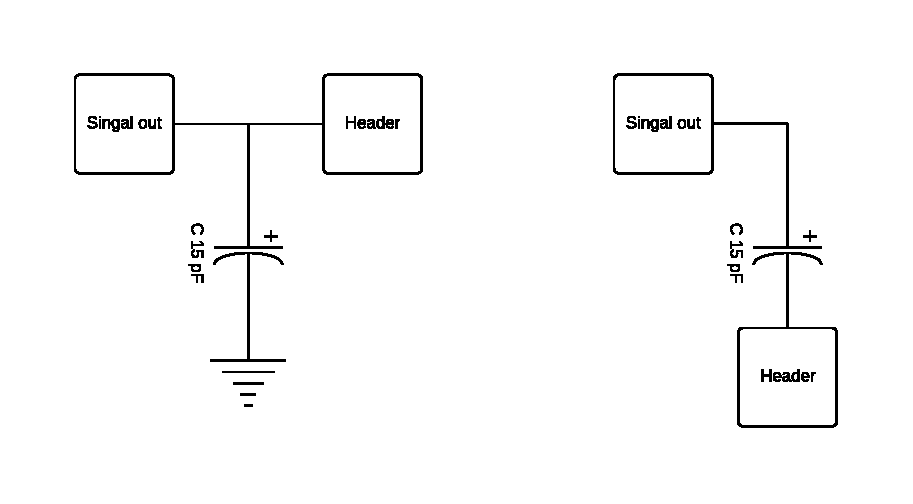
\includegraphics[width=0.65\textwidth]{../pcb/assets/pcb-clock.pdf}
    \label{fig:pcb-clock}
    \caption{On the left: How the clock from the FPGA is supposed to be connected.
             On the right: how it got connected on the PCB.}
\end{figure}

Because of this, the clock did not work.
Our solution to this problem was to solder together the place where the first capacitor was to make room for the signal to flow freely to the header.
Afterwards a through-hole version of the same capacitor was placed on one of the soldering pads and the other end grounded.
This caused the circuit on the board to fully match up with the correct circuit from the data sheet.

\end{document}
